\begin{center}
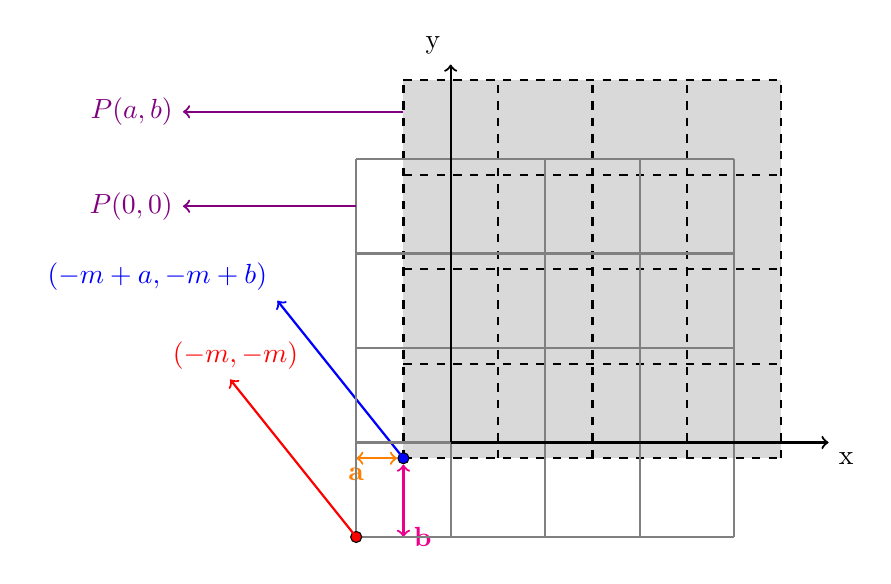
\begin{tikzpicture}[scale=0.4]

    \fill[gray!30] (0,0) rectangle (12,12);

   

    % Second Grid (dashed), positioned 2 units left and 3 units below
   
    \draw[step=3cm,black,dashed, thick] (0,0) grid (12,12);
    \filldraw[fill=blue] circle (5pt) ;
    \draw[orange, <->, thick] (-0.2, 0) -- (-1.5, 0) node[below] {\textbf{a}};
    \draw[magenta, <->, thick] (0, -0.2) -- (0, -2.5) node[right] {\textbf{b}};
    \draw[blue, ->, thick] (0, 0) -- (-4, 5) node[anchor=south east] {\textbf{ $(-m+a,-m+b)$}};

    
    

    \begin{scope}[xshift=-1.5cm, yshift=-2.5cm]
        \draw[step=3cm,gray, thick] (0,0) grid (12,12);
        \filldraw[fill=red] circle (5pt) ;
        \draw[red, ->, thick] (0, 0) -- (-4, 5) node[above] {\textbf{ $(-m,-m)$}};
        \draw[thick,->,black] (3,3) -- (15,3) node[anchor=north west] {x};
        \draw[thick,->,black] (3,3) -- (3,15) node[anchor=south east] {y};
    \end{scope}

    \draw[thick,->,violet] (0,11) -- (-7,11) node[left] {$P(a,b)$};
    \draw[thick,->,violet] (-1.5,8) -- (-7,8) node[left] {$P(0,0)$};

\end{tikzpicture}
\end{center}

%\draw[blue, ->, thick] (13.5, 13.5) -- (16, 15) node[right] {\textbf{\textit{\huge $\frac{1}{\sqrt{2}} \times \frac{1}{\sqrt{2}}$}}};